\part{Kitchen}

\chapter{Overview}


\section{Node}


\begin{lstlisting}[language=bash]
$ curl -sL https://deb.nodesource.com/setup_7.x | sudo -E bash -
$ sudo apt-get install -y nodejs
$ node -v
v7.5.0
$ nodejs -v
v7.5.0
$ npm -v
4.1.2
\end{lstlisting}


\section{NPM}

\begin{lstlisting}[language=bash]
$ npm install -g npm@latest
$ npm -v
4.1.2
\end{lstlisting}

进入/path/to/hitour/themes/kitchen安装项目依赖:


\begin{lstlisting}[language=bash]
$ cd /path/to/hitour/themes/kitchen
$ sudo npm i
\end{lstlisting}

\begin{figure}[htbp]
\centering
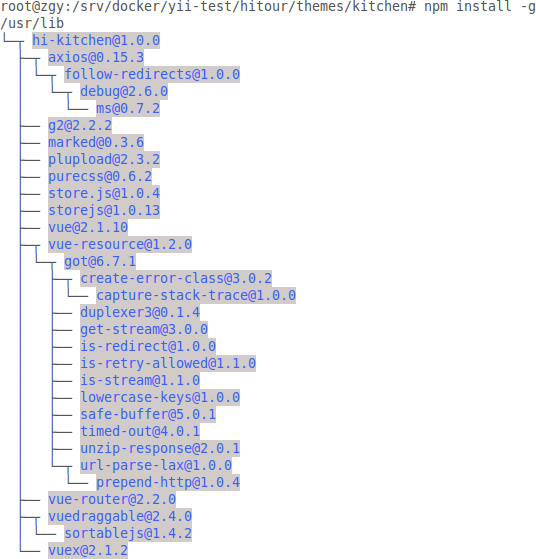
\includegraphics[scale=0.4]{kitchen-dependence.png}
\caption{kitchen项目前端依赖关系}
\end{figure}


创建本地的前端开发服务器配置文件/path/to/hitour/themes/kitchen/config/index.js,index.js的内容如下:

\begin{lstlisting}[language=JavaScript]
var path = require('path')

var common_proxy = {
  //target       : 'http://test.hitour.cc',
  //target       : 'http://sandbox.hitour.cc',
  target: 'http://trial.hitour.cc',
  // target       : 'http://hitour.host',
  changeOrigin: true,
  pathRewrite: {}
};

module.exports = {
  build: {
    env: require('./prod.env'),
    index: path.resolve(__dirname, '../dist/index.html'),
    assetsRoot: path.resolve(__dirname, '../dist'),
    assetsSubDirectory: 'static',
    assetsPublicPath: '/themes/kitchen/dist/',
    productionSourceMap: true,
    productionGzip: false,
    productionGzipExtensions: ['js', 'css']
  },
  dev: {
    env: require('./dev.env'),
    port: 60003,
    assetsSubDirectory: 'static',
    assetsPublicPath: '/',
    proxyTable: {
      '/admin/': common_proxy,
      '/chef/': common_proxy,
      '/themes': common_proxy,
      '/markMi/': common_proxy
    },
    cssSourceMap: false
  }
}
\end{lstlisting}

在/path/to/hitour/themes/kitchen目录下启动本地测试服务器,并且在\url{http://localhost:10003/k/sign\_in}进行测试。

\begin{lstlisting}[language=bash]
$ cd /path/to/hitour/themes/kitchen
$ npm run dev
\end{lstlisting}

如果本地测试通过,可以执行\texttt{npm run build}进行发布。

\begin{lstlisting}[language=bash]
$ cd /path/to/hitour/themes/kitchen
$ npm run build
\end{lstlisting}

注意,在本地或远程服务器做发布之前, 需要确认Yii的路由配置。

\subsection{access}

\begin{lstlisting}[language=bash]

\end{lstlisting}

\subsection{adduser}

\begin{lstlisting}[language=bash]

\end{lstlisting}

\subsection{bin}


\begin{lstlisting}[language=bash]

\end{lstlisting}

\subsection{bugs}


\begin{lstlisting}[language=bash]

\end{lstlisting}

\subsection{c}



\begin{lstlisting}[language=bash]

\end{lstlisting}

\subsection{cache}


\begin{lstlisting}[language=bash]

\end{lstlisting}

\subsection{completion}



\begin{lstlisting}[language=bash]

\end{lstlisting}

\subsection{config}


\begin{lstlisting}[language=bash]
$ npm config list

\end{lstlisting}

\subsection{ddp}


\begin{lstlisting}[language=bash]

\end{lstlisting}

\subsection{dedupe}



\begin{lstlisting}[language=bash]

\end{lstlisting}

\subsection{deprecate}




\begin{lstlisting}[language=bash]

\end{lstlisting}

\subsection{dist-tag}


\begin{lstlisting}[language=bash]

\end{lstlisting}

\subsection{docs}



\begin{lstlisting}[language=bash]

\end{lstlisting}

\subsection{doctor}



\begin{lstlisting}[language=bash]

\end{lstlisting}

\subsection{edit}



\begin{lstlisting}[language=bash]

\end{lstlisting}

\subsection{explore}



\begin{lstlisting}[language=bash]

\end{lstlisting}

\subsection{get}



\begin{lstlisting}[language=bash]

\end{lstlisting}

\subsection{help}



\begin{lstlisting}[language=bash]

\end{lstlisting}

\subsection{help-search}

\begin{lstlisting}[language=bash]

\end{lstlisting}

\subsection{i}


\begin{lstlisting}[language=bash]

\end{lstlisting}

\subsection{init}


\begin{lstlisting}[language=bash]

\end{lstlisting}

\subsection{install}


\begin{lstlisting}[language=bash]

\end{lstlisting}

\subsection{install-test}


\begin{lstlisting}[language=bash]

\end{lstlisting}

\subsection{it}


\begin{lstlisting}[language=bash]

\end{lstlisting}

\subsection{link}


\begin{lstlisting}[language=bash]

\end{lstlisting}

\subsection{list}


\begin{lstlisting}[language=bash]

\end{lstlisting}

\subsection{ln}



\begin{lstlisting}[language=bash]

\end{lstlisting}

\subsection{login}



\begin{lstlisting}[language=bash]

\end{lstlisting}

\subsection{logout}



\begin{lstlisting}[language=bash]

\end{lstlisting}

\subsection{ls}



\begin{lstlisting}[language=bash]

\end{lstlisting}

\subsection{outdated}


\begin{lstlisting}[language=bash]

\end{lstlisting}


\subsection{owner}


\begin{lstlisting}[language=bash]

\end{lstlisting}

\subsection{pack}


\begin{lstlisting}[language=bash]

\end{lstlisting}

\subsection{ping}



\begin{lstlisting}[language=bash]

\end{lstlisting}

\subsection{prefix}


\begin{lstlisting}[language=bash]

\end{lstlisting}

\subsection{prune}

\begin{lstlisting}[language=bash]

\end{lstlisting}

\subsection{publish}


\begin{lstlisting}[language=bash]

\end{lstlisting}

\subsection{rb}



\begin{lstlisting}[language=bash]

\end{lstlisting}

\subsection{rebuild}




\begin{lstlisting}[language=bash]

\end{lstlisting}

\subsection{repo}


\begin{lstlisting}[language=bash]

\end{lstlisting}

\subsection{restart}

\begin{lstlisting}[language=bash]

\end{lstlisting}

\subsection{root}


\begin{lstlisting}[language=bash]

\end{lstlisting}

\subsection{run}



\begin{lstlisting}[language=bash]

\end{lstlisting}

\subsection{run-script}


\begin{lstlisting}[language=bash]

\end{lstlisting}

\subsection{s}


\begin{lstlisting}[language=bash]

\end{lstlisting}


\subsection{se}


\begin{lstlisting}[language=bash]

\end{lstlisting}

\subsection{search}



\begin{lstlisting}[language=bash]

\end{lstlisting}

\subsection{set}



\begin{lstlisting}[language=bash]

\end{lstlisting}

\subsection{shrinkwrap}




\begin{lstlisting}[language=bash]

\end{lstlisting}

\subsection{star}




\begin{lstlisting}[language=bash]

\end{lstlisting}

\subsection{stars}

\begin{lstlisting}[language=bash]

\end{lstlisting}

\subsection{start}


\begin{lstlisting}[language=bash]

\end{lstlisting}

\subsection{stop}



\begin{lstlisting}[language=bash]

\end{lstlisting}


\subsection{t}


\begin{lstlisting}[language=bash]

\end{lstlisting}

\subsection{team}



\begin{lstlisting}[language=bash]

\end{lstlisting}

\subsection{test}




\begin{lstlisting}[language=bash]

\end{lstlisting}

\subsection{tst}






\begin{lstlisting}[language=bash]

\end{lstlisting}

\subsection{un}

\begin{lstlisting}[language=bash]

\end{lstlisting}

\subsection{uninstall}


\begin{lstlisting}[language=bash]

\end{lstlisting}

\subsection{unpublish}



\begin{lstlisting}[language=bash]

\end{lstlisting}

\subsection{unstar}




\begin{lstlisting}[language=bash]

\end{lstlisting}

\subsection{up}



\begin{lstlisting}[language=bash]

\end{lstlisting}

\subsection{update}



\begin{lstlisting}[language=bash]

\end{lstlisting}

\subsection{v}





\begin{lstlisting}[language=bash]

\end{lstlisting}

\subsection{version}

\begin{lstlisting}[language=bash]
$ npm version
{
  npm: '4.1.2',
  ares: '1.10.1-DEV',
  cldr: '29.0',
  http_parser: '2.7.0',
  icu: '57.1',
  modules: '51',
  node: '7.5.0',
  openssl: '1.0.2k',
  tz: '2016b',
  unicode: '8.0',
  uv: '1.10.2',
  v8: '5.4.500.48',
  zlib: '1.2.8' 
}
\end{lstlisting}

\subsection{view}


\begin{lstlisting}[language=bash]
$ npm view vue version
2.1.10
$ npm view vue-cli version
2.8.1
$ npm view vue-router version
2.20
$ npm view vue-resource version
1.2.0
$ npm view webpack version
2.2.1
\end{lstlisting}

\subsection{whoami}



\begin{lstlisting}[language=bash]

\end{lstlisting}




\begin{lstlisting}[language=bash]

\end{lstlisting}




\begin{lstlisting}[language=bash]

\end{lstlisting}




\begin{lstlisting}[language=bash]

\end{lstlisting}



\section{CNPM}

可以使用定制的 cnpm (gzip 压缩支持) 命令行工具代替默认的 npm:

\begin{lstlisting}[language=bash]
$ npm install -g cnpm --registry=https://registry.npm.taobao.org
\end{lstlisting}

或者直接通过添加 npm 参数 alias 一个新命令:

\begin{lstlisting}[language=bash]
$ alias cnpm="npm --registry=https://registry.npm.taobao.org \
--cache=$HOME/.npm/.cache/cnpm \
--disturl=https://npm.taobao.org/dist \
--userconfig=$HOME/.cnpmrc"

# Or alias it in .bashrc or .zshrc
$ echo '\n#alias for cnpm\nalias cnpm="npm --registry=https://registry.npm.taobao.org \
  --cache=$HOME/.npm/.cache/cnpm \
  --disturl=https://npm.taobao.org/dist \
  --userconfig=$HOME/.cnpmrc"' >> ~/.zshrc && source ~/.zshrc
\end{lstlisting}

从 registry.npm.taobao.org 安装模块时,如果发现安装的模块还没有同步过来, 淘宝 NPM 会自动在后台进行同步, 并且会让用户从官方 NPM registry.npmjs.org 进行安装. 下次再安装这个模块的时候, 就会直接从 淘宝 NPM 安装了。


\begin{lstlisting}[language=bash]
$ cnpm install [name]
\end{lstlisting}

直接通过 sync 命令马上同步一个模块, 注意只有 cnpm 命令行才有此功能:

\begin{lstlisting}[language=bash]
$ cnpm sync connect
\end{lstlisting}

可以直接通过 web 方式来同步: /sync/connect

\begin{lstlisting}[language=bash]
$ open https://npm.taobao.org/sync/connect
\end{lstlisting}


cnpm支持 npm 除了 publish 之外的所有命令, 例如:

\begin{lstlisting}[language=bash]
$ cnpm info connect
\end{lstlisting}


\section{Nginx}




\begin{lstlisting}[language=bash]

\end{lstlisting}


\begin{lstlisting}[language=bash]

\end{lstlisting}


\begin{lstlisting}[language=bash]

\end{lstlisting}

\section{Webpack}


\begin{lstlisting}[language=bash]
$ sudo npm i webpack -g
/usr/bin/webpack -> /usr/lib/node_modules/webpack/bin/webpack.js
$ webpack -v
2.2.1
\end{lstlisting}

\chapter{Kitchen}

index.html的内容如下:


\begin{lstlisting}[language=HTML]
<!DOCTYPE html>
<html>
  <head>
    <meta charset="utf-8">
    <title>hi-kitchen</title>
  </head>
  <body>
    <div id="app"></div>
    <!-- built files will be auto injected -->
  </body>
</html>
\end{lstlisting}


\section{build}


\subsection{build.js}


\begin{lstlisting}[language=bash]
// https://github.com/shelljs/shelljs
require('shelljs/global')
env.NODE_ENV = 'production'

var path = require('path')
var config = require('../config')
var ora = require('ora')
var webpack = require('webpack')
var webpackConfig = require('./webpack.prod.conf')

console.log(
  '  Tip:\n' +
  '  Built files are meant to be served over an HTTP server.\n' +
  '  Opening index.html over file:// won\'t work.\n'
)

var spinner = ora('building for production...')
spinner.start()

var assetsPath = path.join(config.build.assetsRoot, config.build.assetsSubDirectory)
rm('-rf', assetsPath)
mkdir('-p', assetsPath)
cp('-R', 'static/*', assetsPath)

webpack(webpackConfig, function (err, stats) {
  spinner.stop()
  if (err) throw err
  process.stdout.write(stats.toString({
    colors: true,
    modules: false,
    children: false,
    chunks: false,
    chunkModules: false
  }) + '\n')
})
\end{lstlisting}

\subsection{dev-client.js}


\begin{lstlisting}[language=bash]
/* eslint-disable */
require('eventsource-polyfill')
var hotClient = require('webpack-hot-middleware/client?noInfo=true&reload=true')

hotClient.subscribe(function (event) {
  if (event.action === 'reload') {
    window.location.reload()
  }
})
\end{lstlisting}


\subsection{dev-server.js}


\begin{lstlisting}[language=bash]
var config = require('../config')
if (!process.env.NODE_ENV) process.env.NODE_ENV = config.dev.env
var path = require('path')
var express = require('express')
var webpack = require('webpack')
var opn = require('opn')
var proxyMiddleware = require('http-proxy-middleware')
var webpackConfig = require('./webpack.dev.conf')

// default port where dev server listens for incoming traffic
var port = process.env.PORT || config.dev.port
// Define HTTP proxies to your custom API backend
// https://github.com/chimurai/http-proxy-middleware
var proxyTable = config.dev.proxyTable

var app = express()
var compiler = webpack(webpackConfig)

var devMiddleware = require('webpack-dev-middleware')(compiler, {
  publicPath: webpackConfig.output.publicPath,
  stats: {
    colors: true,
    chunks: false
  }
})

var hotMiddleware = require('webpack-hot-middleware')(compiler)
// force page reload when html-webpack-plugin template changes
compiler.plugin('compilation', function (compilation) {
  compilation.plugin('html-webpack-plugin-after-emit', function (data, cb) {
    hotMiddleware.publish({ action: 'reload' })
    cb()
  })
})

// proxy api requests
Object.keys(proxyTable).forEach(function (context) {
  var options = proxyTable[context]
  if (typeof options === 'string') {
    options = { target: options }
  }
  app.use(proxyMiddleware(context, options))
})

// handle fallback for HTML5 history API
app.use(require('connect-history-api-fallback')())

// serve webpack bundle output
app.use(devMiddleware)

// enable hot-reload and state-preserving
// compilation error display
app.use(hotMiddleware)

// serve pure static assets
var staticPath = path.posix.join(config.dev.assetsPublicPath, config.dev.assetsSubDirectory)
app.use(staticPath, express.static('./static'))

module.exports = app.listen(port, function (err) {
  if (err) {
    console.log(err)
    return
  }
  var uri = 'http://localhost:' + port
  console.log('Listening at ' + uri + '\n')
  opn(uri)
})
\end{lstlisting}

\section{config}

\subsection{dev.env.js}


\begin{lstlisting}[language=bash]
var merge = require('webpack-merge')
var prodEnv = require('./prod.env')

module.exports = merge(prodEnv, {
  NODE_ENV: '"development"'
})
\end{lstlisting}


\subsection{prod.env.js}



\begin{lstlisting}[language=bash]
module.exports = {
  NODE_ENV: '"production"'
}
\end{lstlisting}

\subsection{index.js}

\begin{lstlisting}[language=bash]
// see http://vuejs-templates.github.io/webpack for documentation.
var path = require('path')

var common_proxy = {
  //target       : 'http://test.hitour.cc',
  //target       : 'http://sandbox.hitour.cc',
  target: 'http://trial.hitour.cc',
  // target       : 'http://hitour.host',
  changeOrigin: true,
  pathRewrite: {}
};

module.exports = {
  build: {
    env: require('./prod.env'),
    index: path.resolve(__dirname, '../dist/index.html'),
    assetsRoot: path.resolve(__dirname, '../dist'),
    assetsSubDirectory: 'static',
    assetsPublicPath: '/themes/kitchen/dist/',
    productionSourceMap: true,
    // Gzip off by default as many popular static hosts such as
    // Surge or Netlify already gzip all static assets for you.
    // Before setting to `true`, make sure to:
    // npm install --save-dev compression-webpack-plugin
    productionGzip: false,
    productionGzipExtensions: ['js', 'css']
  },
  dev: {
    env: require('./dev.env'),
    port: 60003,
    assetsSubDirectory: 'static',
    assetsPublicPath: '/',
    proxyTable: {
      '/admin/': common_proxy,
      '/chef/': common_proxy,
      '/themes': common_proxy,
      '/markMi/': common_proxy
    },
    // CSS Sourcemaps off by default because relative paths are "buggy"
    // with this option, according to the CSS-Loader README
    // (https://github.com/webpack/css-loader#sourcemaps)
    // In our experience, they generally work as expected,
    // just be aware of this issue when enabling this option.
    cssSourceMap: false
  }
}
\end{lstlisting}

\section{views}


\subsection{\_components}


\begin{lstlisting}[language=bash]

\end{lstlisting}



\begin{lstlisting}[language=bash]

\end{lstlisting}


\subsection{\_router}



\begin{lstlisting}[language=bash]

\end{lstlisting}



\begin{lstlisting}[language=bash]

\end{lstlisting}



\subsection{\_store}


\begin{lstlisting}[language=bash]

\end{lstlisting}



\begin{lstlisting}[language=bash]

\end{lstlisting}



\subsection{\_styles}



\begin{lstlisting}[language=bash]

\end{lstlisting}



\begin{lstlisting}[language=bash]

\end{lstlisting}


\subsection{\_utils}




\begin{lstlisting}[language=bash]

\end{lstlisting}



\begin{lstlisting}[language=bash]

\end{lstlisting}



\chapter{\_components}


\begin{lstlisting}[language=bash]

\end{lstlisting}



\begin{lstlisting}[language=bash]

\end{lstlisting}



\chapter{\_router}


\section{index.js}



\begin{lstlisting}[language=bash]

\end{lstlisting}



\begin{lstlisting}[language=bash]

\end{lstlisting}



\section{library.js}



\begin{lstlisting}[language=bash]

\end{lstlisting}



\begin{lstlisting}[language=bash]

\end{lstlisting}


\section{operation.js}




\begin{lstlisting}[language=bash]

\end{lstlisting}



\begin{lstlisting}[language=bash]

\end{lstlisting}



\section{order.js}


\begin{lstlisting}[language=bash]

\end{lstlisting}



\begin{lstlisting}[language=bash]

\end{lstlisting}


\section{resource.js}



\begin{lstlisting}[language=bash]

\end{lstlisting}



\begin{lstlisting}[language=bash]

\end{lstlisting}


\section{sale\_rule.js}




\begin{lstlisting}[language=bash]

\end{lstlisting}



\begin{lstlisting}[language=bash]

\end{lstlisting}






\begin{lstlisting}[language=bash]

\end{lstlisting}



\begin{lstlisting}[language=bash]

\end{lstlisting}






\begin{lstlisting}[language=bash]

\end{lstlisting}



\begin{lstlisting}[language=bash]

\end{lstlisting}






\begin{lstlisting}[language=bash]

\end{lstlisting}



\begin{lstlisting}[language=bash]

\end{lstlisting}






\begin{lstlisting}[language=bash]

\end{lstlisting}



\begin{lstlisting}[language=bash]

\end{lstlisting}






\begin{lstlisting}[language=bash]

\end{lstlisting}



\begin{lstlisting}[language=bash]

\end{lstlisting}






\begin{lstlisting}[language=bash]

\end{lstlisting}



\begin{lstlisting}[language=bash]

\end{lstlisting}





\begin{lstlisting}[language=bash]

\end{lstlisting}



\begin{lstlisting}[language=bash]

\end{lstlisting}






\begin{lstlisting}[language=bash]

\end{lstlisting}



\begin{lstlisting}[language=bash]

\end{lstlisting}






\begin{lstlisting}[language=bash]

\end{lstlisting}



\begin{lstlisting}[language=bash]

\end{lstlisting}






\begin{lstlisting}[language=bash]

\end{lstlisting}



\begin{lstlisting}[language=bash]

\end{lstlisting}






\begin{lstlisting}[language=bash]

\end{lstlisting}



\begin{lstlisting}[language=bash]

\end{lstlisting}






\begin{lstlisting}[language=bash]

\end{lstlisting}



\begin{lstlisting}[language=bash]

\end{lstlisting}






\begin{lstlisting}[language=bash]

\end{lstlisting}



\begin{lstlisting}[language=bash]

\end{lstlisting}






\begin{lstlisting}[language=bash]

\end{lstlisting}



\begin{lstlisting}[language=bash]

\end{lstlisting}





\begin{lstlisting}[language=bash]

\end{lstlisting}



\begin{lstlisting}[language=bash]

\end{lstlisting}






\begin{lstlisting}[language=bash]

\end{lstlisting}



\begin{lstlisting}[language=bash]

\end{lstlisting}






\begin{lstlisting}[language=bash]

\end{lstlisting}



\begin{lstlisting}[language=bash]

\end{lstlisting}






\begin{lstlisting}[language=bash]

\end{lstlisting}



\begin{lstlisting}[language=bash]

\end{lstlisting}






\begin{lstlisting}[language=bash]

\end{lstlisting}



\begin{lstlisting}[language=bash]

\end{lstlisting}






\begin{lstlisting}[language=bash]

\end{lstlisting}



\begin{lstlisting}[language=bash]

\end{lstlisting}






\begin{lstlisting}[language=bash]

\end{lstlisting}



\begin{lstlisting}[language=bash]

\end{lstlisting}






\begin{lstlisting}[language=bash]

\end{lstlisting}



\begin{lstlisting}[language=bash]

\end{lstlisting}





\begin{lstlisting}[language=bash]

\end{lstlisting}



\begin{lstlisting}[language=bash]

\end{lstlisting}






\begin{lstlisting}[language=bash]

\end{lstlisting}



\begin{lstlisting}[language=bash]

\end{lstlisting}






\begin{lstlisting}[language=bash]

\end{lstlisting}



\begin{lstlisting}[language=bash]

\end{lstlisting}






\begin{lstlisting}[language=bash]

\end{lstlisting}



\begin{lstlisting}[language=bash]

\end{lstlisting}






\begin{lstlisting}[language=bash]

\end{lstlisting}



\begin{lstlisting}[language=bash]

\end{lstlisting}






\begin{lstlisting}[language=bash]

\end{lstlisting}



\begin{lstlisting}[language=bash]

\end{lstlisting}






\begin{lstlisting}[language=bash]

\end{lstlisting}



\begin{lstlisting}[language=bash]

\end{lstlisting}







\chapter{分组接口}


\section{/chef/api/operation/productGroup/Group}


\subsection{GET}

获取分组详情

URL:\url{/chef/api/operation/productGroup/Group}





\begin{longtable}{|m{50pt}|m{40pt}|m{50pt}|m{50pt}|}
%head
\multicolumn{4}{r}{}
\tabularnewline\hline
字段&类型&必填&备注
\endhead
%endhead

%firsthead
\caption{获取分组详情接口-请求参数}\\
\hline
字段&类型&必填&备注
\endfirsthead
%endfirsthead

%foot
\multicolumn{4}{r}{}
\endfoot
%endfoot

%lastfoot
\endlastfoot
%endlastfoot
\hline
group\_id&int&是&分组ID\\
\hline
\end{longtable}

\begin{lstlisting}[language=JavaScript]
{
  "code": 200,
  "msg": "Ok.",
  "data": {
    "group_id": "19",
    "show_type": "0",
    "title": "扫货扫货qu去首尔",
    "sub_title": "特价机票+酒店",
    "short_desc": "",
    "route_desc": "首尔自由行特价机票酒店,1999起",
    "date_desc": "",
    "pc_image_url": "http://pics.hitour.cc/e969a4546e0228ebe7ed9ffe52319962.png",
    "h5_image_url": "",
    "icon_image_url": "",
    "start_date": "2016-08-23",
    "end_date": "2016-12-31",
    "status": "1",
    "type": "1",
    "group_dests": [
      {
        "id": "27",
        "group_id": "19",
        "dest_code": "1",
        "name": "华南",
        "type": "1",
        "display_order": "5"
      }
   ],
    "group_locations": [
      {
        "label_id": "1",
        "group_id": "19",
        "city_code": "SEL",
        "type": "3",
        "city": {
          "country_code": "KR",
          "city_code": "SEL",
          "iata_code": "SEL",
          "cn_name": "首尔",
          "en_name": "Seoul",
          "pinyin": "shou er",
          "timezone": "+9:00",
          "has_product": "1",
          "has_online_product": "1",
          "top_search": "[{\"value\":\"\\u4e50\\u5929\\u4e16\\u754c\",\"display_order\":1},{\"value\":\"\\u6c11\\u4fd7\",\"display_order\":2},{\"value\":\"\\u4e71\\u6253\\u79c0\",\"display_order\":3},{\"value\":\"\\u660e\\u6d1e\",\"display_order\":4},{\"value\":\"\\u6c5d\\u77e3\\u5c9b\",\"display_order\":5},{\"value\":\"\\u4e1c\\u5927\\u95e8\",\"display_order\":6}]",
          "data_level": "2",
          "show_in_country": "0",
          "link_url": "/South_Korea/Seoul",
          "link_url_m": "/mobile#/city/SEL",
          "city_name": "Seoul",
          "country_name": "South_Korea",
          "country_cn_name": "韩国"
        }
      }
    ],
    "group_products": [
         {
        "id": "44",
        "group_id": "19",
        "product_id": "8837",
        "display_order": "8",
        "product_description": {
          "name": "【秋游季】上海直飞首尔4-5天机酒自由行•五星航空韩亚往返机票+全程热销酒店套餐任选 赠接机半日游/首尔1日游/自由行大礼包",
          "product_id": "8837",
          "language_id": "2"
        }
      }
    ]
  }
}
\end{lstlisting}


\subsection{POST}

新增分组

URL:\url{/chef/api/operation/productGroup/Group}



\begin{longtable}{|m{80pt}|m{40pt}|m{50pt}|m{150pt}|}
%head
\multicolumn{4}{r}{}
\tabularnewline\hline
字段&类型&必填&备注
\endhead
%endhead

%firsthead
\caption{新增分组接口-请求参数}\\
\hline
字段&类型&必填&备注
\endfirsthead
%endfirsthead

%foot
\multicolumn{4}{r}{}
\endfoot
%endfoot

%lastfoot
\endlastfoot
%endlastfoot
\hline
title			&string	&是	&唯一\\
\hline
sub\_title	&string	&否	&副标题\\
\hline
short\_desc	&string	&否	&短标题\\
\hline
route\_desc	&string	&是	&专题线路\\
\hline
date\_desc	&string	&是	&专题日期\\
\hline
pc\_image\_url&string	&否	&\\
\hline
h5\_image\_url&string	&否	&\\
\hline
icon\_image\_url&string&否	&\\
\hline
start\_date	&date	&是	&\\
\hline
end\_date	&date	&是	&\\
\hline
type			&int		&是	&1普通分组,2是父级分组\\
\hline
city\_code	&array	&是	&城市\\
\hline
\end{longtable}


\begin{lstlisting}[language=JavaScript]
{
  "code": 200,
  "msg": "Ok.",
  "data": {
    "show_type": 0,
    "title": "扫货扫货401",
    "sub_title": "lalaa",
    "short_desc": "",
    "route_desc": "",
    "date_desc": "",
    "start_date": "0000-00-00",
    "end_date": "0000-00-00",
    "status": 0,
    "type": 1,
    "group_id": "49",
    "pc_image_url": null,
    "h5_image_url": null,
    "icon_image_url": null,
    "group_locations": [
      {
        "label_id": "1",
        "group_id": "19",
        "city_code": "SEL",
        "type": "3",
        "city": {
          "country_code": "KR",
          "city_code": "SEL",
          "iata_code": "SEL",
          "cn_name": "首尔",
          "en_name": "Seoul",
          "pinyin": "shou er",
          "timezone": "+9:00",
          "has_product": "1",
          "has_online_product": "1",
          "top_search": "[{\"value\":\"\\u4e50\\u5929\\u4e16\\u754c\",\"display_order\":1},{\"value\":\"\\u6c11\\u4fd7\",\"display_order\":2},{\"value\":\"\\u4e71\\u6253\\u79c0\",\"display_order\":3},{\"value\":\"\\u660e\\u6d1e\",\"display_order\":4},{\"value\":\"\\u6c5d\\u77e3\\u5c9b\",\"display_order\":5},{\"value\":\"\\u4e1c\\u5927\\u95e8\",\"display_order\":6}]",
          "data_level": "2",
          "show_in_country": "0",
          "link_url": "/South_Korea/Seoul",
          "link_url_m": "/mobile#/city/SEL",
          "city_name": "Seoul",
          "country_name": "South_Korea",
          "country_cn_name": "韩国"
        }
      }
    ],
  }
}
\end{lstlisting}


\subsection{PUT}

更新分组

URL:\url{/chef/api/operation/productGroup/Group}


\begin{longtable}{|m{80pt}|m{40pt}|m{50pt}|m{150pt}|}
%head
\multicolumn{4}{r}{}
\tabularnewline\hline
字段&类型&必填&备注
\endhead
%endhead

%firsthead
\caption{更新分组接口-请求参数}\\
\hline
字段&类型&必填&备注
\endfirsthead
%endfirsthead

%foot
\multicolumn{4}{r}{}
\endfoot
%endfoot

%lastfoot
\endlastfoot
%endlastfoot
\hline
group\_id	&int		&是	&\\
\hline
title			&string	&否	&唯一\\
\hline
sub\_title	&string	&否	&副标题\\
\hline
short\_desc	&string	&否	&短标题\\
\hline
route\_desc	&string	&是	&专题线路\\
\hline
date\_desc	&string	&是	&专题日期\\
\hline
pc\_image\_url&string	&否	&\\
\hline
h5\_image\_url&string	&否	&\\
\hline
icon\_image\_url&string&否	&\\
\hline
start\_date	&date	&否	&\\
\hline
end\_date	&date	&否	&\\
\hline
type			&int		&否	&1普通分组,2是父级分组\\
\hline
city\_code	&array	&否	&城市\\
\hline
\end{longtable}

\begin{lstlisting}[language=JavaScript]
{
  "code": 200,
  "msg": "Ok.",
  "data": {
    "show_type": 0,
    "title": "扫货扫货401",
    "sub_title": "lalaa",
    "short_desc": "",
    "route_desc": "",
    "date_desc": "",
    "start_date": "0000-00-00",
    "end_date": "0000-00-00",
    "status": 0,
    "type": 1,
    "group_id": "49",
    "pc_image_url": null,
    "h5_image_url": null,
    "icon_image_url": null,
    "group_locations": [
      {
        "label_id": "1",
        "group_id": "19",
        "city_code": "SEL",
        "type": "3",
        "city": {
          "country_code": "KR",
          "city_code": "SEL",
          "iata_code": "SEL",
          "cn_name": "首尔",
          "en_name": "Seoul",
          "pinyin": "shou er",
          "timezone": "+9:00",
          "has_product": "1",
          "has_online_product": "1",
          "top_search": "[{\"value\":\"\\u4e50\\u5929\\u4e16\\u754c\",\"display_order\":1},{\"value\":\"\\u6c11\\u4fd7\",\"display_order\":2},{\"value\":\"\\u4e71\\u6253\\u79c0\",\"display_order\":3},{\"value\":\"\\u660e\\u6d1e\",\"display_order\":4},{\"value\":\"\\u6c5d\\u77e3\\u5c9b\",\"display_order\":5},{\"value\":\"\\u4e1c\\u5927\\u95e8\",\"display_order\":6}]",
          "data_level": "2",
          "show_in_country": "0",
          "link_url": "/South_Korea/Seoul",
          "link_url_m": "/mobile#/city/SEL",
          "city_name": "Seoul",
          "country_name": "South_Korea",
          "country_cn_name": "韩国"
        }
      }
    ],
  }
}
\end{lstlisting}



\subsection{DELETE}

删除分组

URL:\url{/chef/api/operation/productGroup/Group}


\begin{longtable}{|m{50pt}|m{40pt}|m{50pt}|m{50pt}|}
%head
\multicolumn{4}{r}{}
\tabularnewline\hline
字段&类型&必填&备注
\endhead
%endhead

%firsthead
\caption{删除分组接口-请求参数}\\
\hline
字段&类型&必填&备注
\endfirsthead
%endfirsthead

%foot
\multicolumn{4}{r}{}
\endfoot
%endfoot

%lastfoot
\endlastfoot
%endlastfoot
\hline
group\_id&int&是&分组ID\\
\hline
\end{longtable}

\begin{lstlisting}[language=JavaScript]
{
  "code": 200,
  "msg": "Ok.",
}
\end{lstlisting}


